% Header: Here are all packages used and some additional definitions
%%%%%%%%%%%%%%%%%%%%%%%%%%%%%%%%%%%%%%%%%%%%%%%%%%%%%%%%%%%%%%%%%%%

\documentclass[11pt,a4paper]{article}
\usepackage[margin=2.5cm]{geometry}
\usepackage[onehalfspacing]{setspace}
\usepackage{graphicx} % zum Einbinden von Graphiken
\usepackage[breaklinks=true,colorlinks=true,linkcolor=blue,urlcolor=blue,citecolor=blue]{hyperref} % f. Referenzen
\usepackage{amsmath,amsthm,amssymb} % Mathematik Umgebung 
\usepackage{icomma} % Intelligentes Komma, das den richtigen Abstand zwischen Dezimalzahlen als auch in Formeln wählt.
%\usepackage[ngerman]{babel} % Deutsche Bezeichnungen bei Inhaltsangabe etc
\usepackage[T1]{fontenc}    % andere Schriftsatzkodierung für richtige Silbentrennung bei Umlauten
\usepackage[locale = DE,space-before-unit=true,per-mode = symbol]{siunitx} % Bessere Einheiten
\usepackage{placeins} % Definiert den Befehl “\FloatBarrier”, der die Ausgabe der davor eingebundenen Bilder erzwingt, befor der Text weiter geht. (Mit vorsicht zu verwenden)
\usepackage[natbib,abbreviate=true,doi=false,style=numeric-comp,giveninits=true,sorting=none]{biblatex} % Modernes Paket zur Erzeugung von Bibliografien (benötigt biber!)

\addbibresource{MyBibliography.bib} % Ort der .bib Datei, die die Datenbank für Literatur/Referenzen enthält.

\graphicspath{{Bilder/}}

\DeclareSIUnit{\dBm}{dBm}
\DeclareSIUnit[per-mode=reciprocal]\WN{\per\centi\meter}


\usepackage[backend=biber, style=numeric, sorting=none, autocite = superscript, maxnames = 10]{biblatex}
\addbibresource{references.bib}

\AtBeginBibliography{\renewbibmacro*{begentry}{\printnames{author}}}
\AtEveryBibitem{\clearfield{note}}

\setlength{\bibhang}{1em}
\defbibenvironment{bibliography}
  {\list
     {\printtext[labelnumberwidth]{%
        \printfield{labelprefix}%
        \printfield{labelnumber}}}
     {\setlength{\labelwidth}{\labelnumberwidth}%
     \setlength{\leftmargin}{\bibhang}
     % \setlength{\leftmargin}{\labelwidth}%
      \setlength{\labelsep}{\biblabelsep}%
      \setlength{\itemsep}{\bibitemsep}%
      \setlength{\parsep}{\bibparsep}%
      \addtolength{\leftmargin}{\labelsep}%
      \setlength{\itemindent}{-\bibhang}
      %\setlength{\itemindent}{0pt}%
      \renewcommand*{\makelabel}[1]{\hss##1}%
      \raggedright}}
  {\endlist}
  {\item}


%%%%%%%%%%%%%%%%%%%%%%%%%%%%%%%%%%%%%%%%%%%%%%%%%%%%%%%%%%%%%%%%%%%
\begin{document}
%
\title{Gut Microbiome in Adult Allo-SCT Patients: Lit Review}
\author{Sophie Huebler \thanks{\href{mailto:sophie.huebler@utah.edu}{sophie.huebler@utah.edu}}}
\date{\today}
\maketitle
%\vfill
\renewcommand\abstractname{Objective}
\section*{\abstractname}
\textit{In adult allo‑HSCT recipients, what is the reported association between gut microbiome diversity/composition and GVHD and related clinical outcomes, and how consistent are findings across studies given methodological heterogeneity?}
\thispagestyle{empty}
%
%
\tableofcontents
\thispagestyle{empty}
\cleardoublepage
\pagenumbering{arabic} 
\newpage
%
%
\section{Strategy}
\label{sec:Strategy}
%
Papers will be sorted into 4 tiers. Tier 4 papers will be examined first, listing out relevant concepts and source papers. Each source paper will be listed for categorization. 
\begin{itemize}
    \item Tier 1 (reanalysis-ready): raw reads + sample mapping/clinical metadata with GVHD outcomes
    \item Tier 2 (salvageable): raw reads exist but metadata incomplete (maybe reconstructable from paper/SRA fields)
    \item Tier 3 (summary-only): no raw reads, but paper reports usable summary stats/effect estimates
    \item Tier 4 (narrative-only): relevant conceptually but no extractable quantitative info; includes scoping reviews
\end{itemize}







%
\section{Tier 4: Narratives}
\label{sec:narratives}
%

\begin{table}[htbp]
\centering
\caption{\label{tab:tier4tab} Narrative and review papers with potentially relevant sources.}

\begin{tabular}{ccccc}
\\ \hline
Paper & Year  & Possible references &   Description & Priority\\
\hline
van Lier & 2023 & 96 (xx) & GVHD pathogenesis and interventions & high \\
Azhar Ud Din & 2025 & 217 (xx)& Therapeutic strategies & low\\
Kaźmierczak-Siedlecka & 2021 & 123 (xx) & FMT  & low\\
Henig & 2020 & 122 (xx) & Clinical & low\\
Kohler & 2019 & 89 (xx) & Immune tolerance & low\\
Shono & 2018 & 169 (xx) & Clinical Review & low\\
Shono & 2015 & 102 (xx) & Clinical Review \\
Chang & 2021 & 111 (xx) & Clinical Review & low \\
Yu & 2020 & 105 (xx) & Clinical and therapeutic & low \\
Fujiwara & 2021 & 173 (xx) & Mechanistic \\
Ciernikova & 2021 &  109 (xx) & Therapeutic strategies \\
Beckman & 2021 & 50 (xx) & Text mining and therapeutic & high (tab) \\
Noor & 2019 & 50 (xx) & Biomarkers and therapeutics & medium \\
Gavriilaki & 2020 & 72 (xx) & Antibiotics & low \\
Wang & 2023 & 62 (xx) & Systematic review and meta & high  \\
Nguyen & 2021 & 85 (xx) & Clinical review & medium \\
Samarkhazan & 2025 & 22 & Therapeutics & high (tab) \\
Kuhat & 2021 & 131 (xx) & Clinical review & low \\
Hong & 2021 & 165 (xx) & Systematic review & high (tab)\\
Yue & 2023 & 183 (xx) & Clinical review & high (tab)\\
Chakraverty & 2021 & 125 (xx) & Therapeutics & low \\
Godefroy & 2025 & 122 (xx) & Mechanistic & high (tab)\\
\hline
Total: &  & xx &  \\

\hline
\end{tabular}
\end{table}

\newpage
\subsection{Samarkhazan2025}
Samarkhazan, H.S., Nouri, S., Maleknia, M., Aghaei, M., 2025. The microbiome in graft-versus-host disease: a tale of two ecosystems. J. Transl. Med. 23, 832. https://doi.org/10.1186/s12967-025-06797-5

\begin{figure}[h]
    \centering
    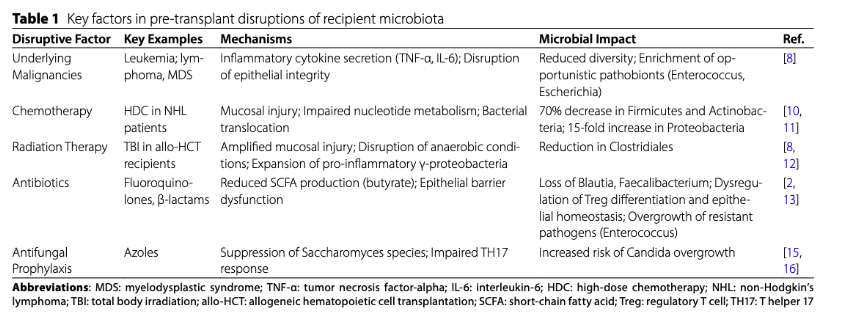
\includegraphics[width=1\linewidth]{Bilder/Samarkhazan2025_Table1.png}
    %\caption{Enter Caption}
    \label{fig:Samarkhazan2025_Table1}
\end{figure}
\begin{itemize}
    \item 8:  Yue X, Zhou H, Wang S, Chen X, Xiao H. Gut microbiota, microbiota-derivedmetabolites, and graft-versus-host disease. Cancer Med. 2024;13(3):e6799.
    \item 10: Montassier E, Gastinne T, Vangay P, et al. Chemotherapy-driven dysbiosis inthe intestinal Microbiome. Aliment Pharmacol Ther. 2015;42(5):515–28.
    \item 11: Liang J, Liu G, Wang W, Xue H. Causal relationships between gut microbiotaand lymphoma: a bidirectional Mendelian randomization study. Front CellInfect Microbiol. 2024;14:1374775.
    \item 12: Rafei H, Jenq RR. Microbiome-intestine cross talk during acute graft-versus-host disease. Blood. 2020;136(4):401–9.
    \item 2: Fredricks DN. The gut microbiota and graft-versus-host disease. J Clin Invest.2019;129(5):1808–17.
    \item 13: Stein-Thoeringer CK, Nichols KB, Lazrak A, et al. Lactose drives Entero-coccus expansion to promote graft-versus-host disease. Science.2019;366(6469):1143–9.
    \item Li Z, Ke X, Zuo D, Wang Z, Fang F, Li B. New insights into the relationshipbetween gut microbiota and radiotherapy for Cancer. Nutrients. 2022;15(1).
    \item 16: Köhler N, Zeiser R. Intestinal microbiota influence immune tolerance postallogeneic hematopoietic cell transplantation and intestinal GVHD. FrontImmunol. 2018;9:3179.
\end{itemize}

\begin{figure}
    \centering
    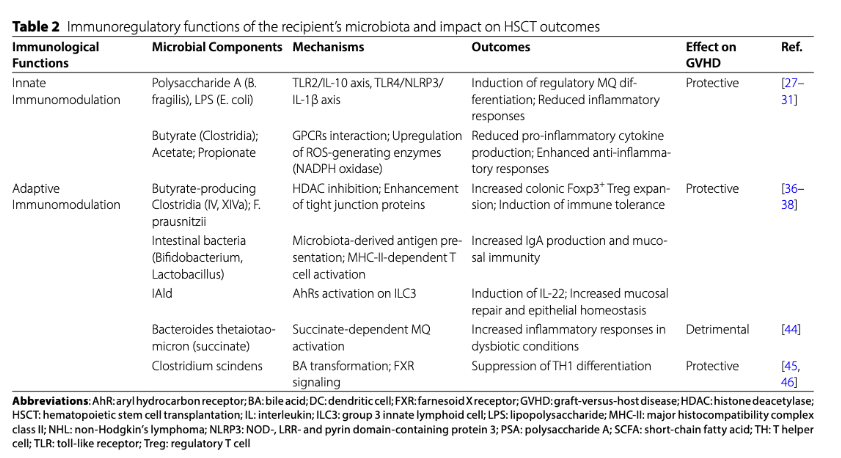
\includegraphics[width=1\linewidth]{Bilder/Samarkhazan2025_Tab2.png}
    \label{fig:Samarkhazan2025_Tab2}
\end{figure}
\begin{itemize}
    \item 27: Biennier S, Fontaine M, Duquenoy A, Schwintner C, Doré J, Corvaia N. Nar-rative review: advancing dysbiosis treatment in Onco-Hematology withMicrobiome-Based therapeutic approach. Microorganisms. 2024;12(11):2256.
    \item 28: Faraci M, Bonaretti C, Dell’Orso G, et al. Association between oral and fecalMicrobiome dysbiosis and treatment complications in pediatric patientsundergoing allogeneic hematopoietic stem cell transplantation. Sci Rep.2024;14(1):6708.
    \item 29: Portincasa P, Bonfrate L, Vacca M et al. Gut microbiota and short chain fattyacids: implications in glucose homeostasis. Int J Mol Sci. 2022;23(3).
    \item 30: Chi M, Jiang T, He X, et al. Role of gut microbiota and oxidative stress in theprogression of Transplant-Related complications following hematopoieticstem cell transplantation. Oxidative Med Cell Longev. 2023;2023(1):3532756.
    \item 31: Rooks MG, Garrett WS. Gut microbiota, metabolites and host immunity. NatRev Immunol. 2016;16(6):341–52.
    \item 36: Takahashi D, Hoshina N, Kabumoto Y, et al. Microbiota-derived butyrate limitsthe autoimmune response by promoting the differentiation of follicularregulatory T cells. EBioMedicine. 2020;58:102913.
    \item 37: Biliński J, Jasiński M, Basak GW. The role of fecal microbiota transplantation inthe treatment of acute Graft-versus-Host disease. Biomedicines. 2022;10(4).
    \item 38: Gavriilaki E, Christoforidi M, Ouranos K, et al. Alteration of gut microbiotacomposition and diversity in acute and/or chronic Graft-versus-Host diseasefollowing hematopoietic stem cell transplantation: A prospective cohortstudy. Int J Mol Sci. 2024;25(11):5789.
    \item 44: Wu J, Wang K, Wang X, Pang Y, Jiang C. The role of the gut Microbiome and itsmetabolites in metabolic diseases. Protein Cell. 2021;12(5):360–73.
    \item 45: Fujiwara H. Crosstalk between intestinal microbiota derived metabolitesand tissues in allogeneic hematopoietic cell transplantation. Front Immunol.2021;12:703298.
    \item 46: Kiriyama Y, Nochi H. The role of gut Microbiota-Derived lithocholic acid,deoxycholic acid and their derivatives on the function and differentiation ofimmune cells. Microorganisms. 2023;11(11).
\end{itemize}


\begin{figure}
    \centering
    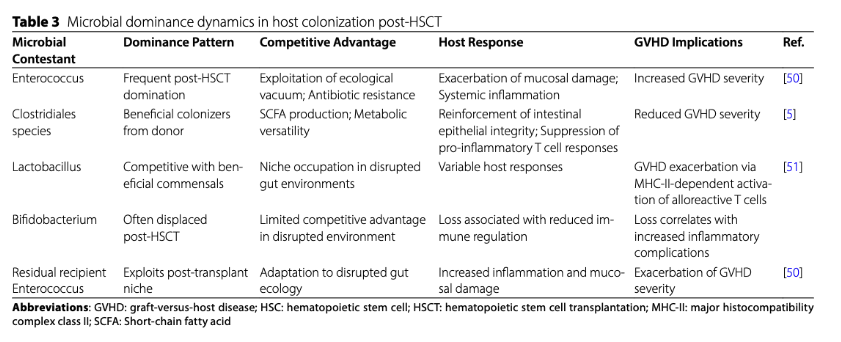
\includegraphics[width=1\linewidth]{Bilder/Samarkhazan2025_Tab3.png}
    \label{fig:Samarkhazan2025_Tab3}
\end{figure}
\begin{itemize}
    \item 50: Khuat LT, Dave M, Murphy WJ. The emerging roles of the gut Microbiomein allogeneic hematopoietic stem cell transplantation. Gut Microbes.2021;13(1):1966262.
    \item 5: Henig I, Yehudai-Ofir D, Zuckerman T. The clinical role of the gut Microbiomeand fecal microbiota transplantation in allogeneic stem cell transplantation.Haematologica. 2021;106(4):933–46.
    \item 51: Kaźmierczak-Siedlecka K, Skonieczna-Żydecka K, Biliński J, et al. Gut Microbi-ome modulation and faecal microbiota transplantation following allogenichematopoietic stem cell transplantation. Cancers (Basel). 2021;13:18.
\end{itemize}

\newpage
\subsection{Hong2021}
Hong, T., Wang, R., Wang, X., Yang, S., Wang, W., Gao, Q., Zhang, X., 2021. Interplay Between the Intestinal Microbiota and Acute Graft-Versus-Host Disease: Experimental Evidence and Clinical Significance. Front. Immunol. 12, 644982. https://doi.org/10.3389/fimmu.2021.644982
\begin{figure}[h]
    \centering
    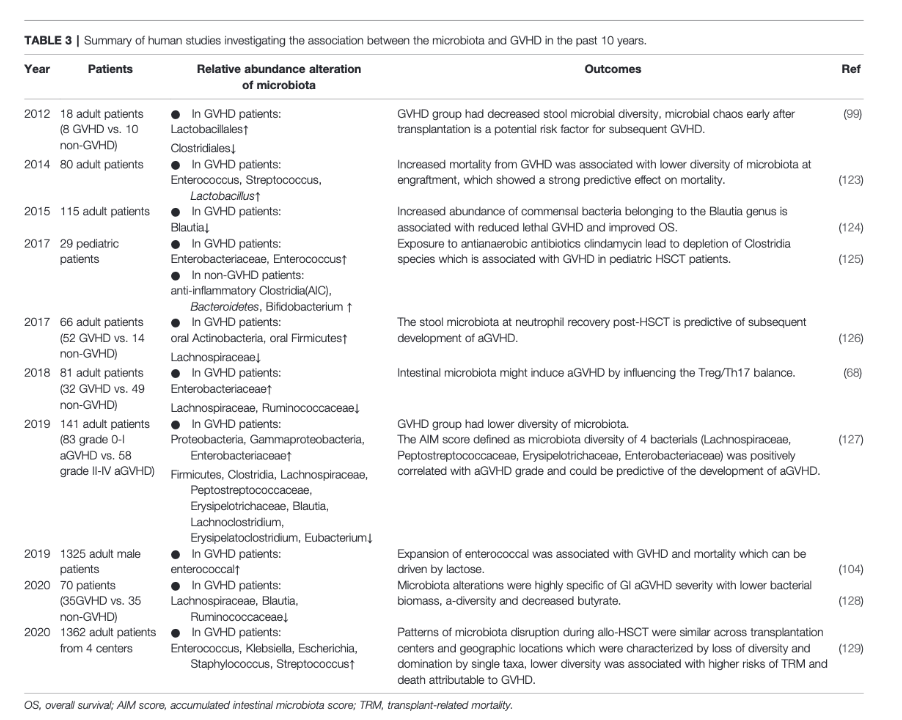
\includegraphics[width=1\linewidth]{Bilder/Hong2021_Tab3.png}
    \label{fig:placeholder}
\end{figure}
\begin{itemize}
    \item 99: Jenq RR, Ubeda C, Taur Y, Menezes CC, Khanin R, Dudakov JA, et al.Regulation of intestinal inflammation by microbiota following allogeneicbone marrow transplantation. J Exp Med (2012) 209(5):903–11. doi:10.1084/jem.20112408 
    \item 123: Taur Y, Jenq RR, Perales MA, Littmann ER, Morjaria S, Ling L, et al. Theeffects of intestinal tract bacterial diversity on mortality following allogeneichematopoietic stem cell transplantation. Blood (2014) 124(7):1174–82. doi:10.1182/blood-2014-02-554725
    \item 124: Jenq RR, Taur Y, Devlin SM, Ponce DM, Goldberg JD, Ahr KF, et al.Intestinal Blautia Is Associated with Reduced Death from Graft-versus-HostDisease. Biol Blood Marrow Transpl (2015) 21(8):1373–83. doi: 10.1016/j.bbmt.2015.04.016
    \item 125: Simms-Waldrip TR, Sunkersett G, Coughlin LA, Savani MR, Arana C, Kim J,et al. Antibiotic-Induced Depletion of Anti-inflammatory Clostridia IsAssociated with the Development of Graft-versus-Host Disease inPediatric Stem Cell Transplantation Patients. Biol Blood Marrow Transpl(2017) 23(5):820–9. doi: 10.1016/j.bbmt.2017.02.004\\
    - Bioproject SRP058320 \\
    - Pediatric \\
    - GVHD but no timing
    \item 126: Golob JL, Pergam SA, Srinivasan S, Fiedler TL, Liu C, Garcia K, et al. StoolMicrobiota at Neutrophil Recovery Is Predictive for Severe Acute Graft vsHost Disease After Hematopoietic Cell Transplantation. Clin Infect Dis(2017) 65(12):1984–91. doi: 10.1093/cid/cix699\\
    - Fred hutch (contact)
    \item 68: Han L, Jin H, Zhou L, Zhang X, Fan Z, Dai M, et al. Intestinal Microbiota atEngraftment Influence Acute Graft-Versus-Host Disease via the Treg/Th17Balance in Allo-HSCT Recipients. Front Immunol (2018) 9:669. doi:10.3389/fimmu.2018.00669\\
    - No mention of public data (china)
    \item 127: Han L, Zhang H, Chen S, Zhou L, Li Y, Zhao K, et al. Intestinal MicrobiotaCan Predict Acute Graft-versus-Host Disease Following AllogeneicHematopoietic Stem Cell Transplantation. Biol Blood Marrow Transpl(2019) 25(10):1944–55. doi: 10.1016/j.bbmt.2019.07.006\\
    - No mention of public data (china)
    \item 104: Stein-Thoeringer CK, Nichols KB, Lazrak A, Docampo MD, Slingerland AE,Slingerland JB, et al. Lactose drives Enterococcus expansion to promotegraft-versus-host disease. Science (2019) 366(6469):1143–9. doi: 10.1126/science.aax3760
    \item 128: Payen M, Nicolis I, Robin M, Michonneau D, Delannoye J, Mayeur C, et al.Functional and phylogenetic alterations in gut microbiome are linked tograft-versus-host disease severity. Blood Adv (2020) 4(9):1824–32. doi:10.1182/bloodadvances.2020001531\\
    - Already contacted, data wherabouts unknown
    \item 129: Peled JU, Gomes ALC, Devlin SM, Littmann ER, Taur Y, Sung AD, et al.Microbiota as Predictor of Mortality in Allogeneic Hematopoietic-CellTransplantation. N Engl J Med (2020) 382(9):822–34. doi: 10.1056/NEJMoa1900623
\end{itemize}

\subsection{Yue2023}

%
\section{Uncategorized}
\label{sec:uncat}

\begin{itemize}
    \item  Yue X, Zhou H, Wang S, Chen X, Xiao H. Gut microbiota, microbiota-derivedmetabolites, and graft-versus-host disease. Cancer Med. 2024;13(3):e6799.\\
    - Review
    \item  Montassier E, Gastinne T, Vangay P, et al. Chemotherapy-driven dysbiosis inthe intestinal Microbiome. Aliment Pharmacol Ther. 2015;42(5):515–28.\\
    - PRJNA257960\\
    - No GVHD outcome
    \item  Liang J, Liu G, Wang W, Xue H. Causal relationships between gut microbiotaand lymphoma: a bidirectional Mendelian randomization study. Front CellInfect Microbiol. 2024;14:1374775.\\
    - Unsure (https://pubmed.ncbi.nlm.nih.gov/38803568/)
    \item Rafei H, Jenq RR. Microbiome-intestine cross talk during acute graft-versus-host disease. Blood. 2020;136(4):401–9.\\
    - Review
    \item  Fredricks DN. The gut microbiota and graft-versus-host disease. J Clin Invest.2019;129(5):1808–17.\\
    - Review
    \item  Stein-Thoeringer CK, Nichols KB, Lazrak A, et al. Lactose drives Entero-coccus expansion to promote graft-versus-host disease. Science.2019;366(6469):1143–9.\\
    - Peled
    \item Li Z, Ke X, Zuo D, Wang Z, Fang F, Li B. New insights into the relationshipbetween gut microbiota and radiotherapy for Cancer. Nutrients. 2022;15(1).\\
    - Therepeutic review
    \item  Köhler N, Zeiser R. Intestinal microbiota influence immune tolerance postallogeneic hematopoietic cell transplantation and intestinal GVHD. FrontImmunol. 2018;9:3179.\\
    - Review (in tier 4 table)
    \item  Biennier S, Fontaine M, Duquenoy A, Schwintner C, Doré J, Corvaia N. Nar-rative review: advancing dysbiosis treatment in Onco-Hematology withMicrobiome-Based therapeutic approach. Microorganisms. 2024;12(11):2256.\\
    - Review
    \item  Faraci M, Bonaretti C, Dell’Orso G, et al. Association between oral and fecalMicrobiome dysbiosis and treatment complications in pediatric patientsundergoing allogeneic hematopoietic stem cell transplantation. Sci Rep.2024;14(1):6708.\\
    - PRJNA929702 \\
    - Pediatric
    \item  Portincasa P, Bonfrate L, Vacca M et al. Gut microbiota and short chain fattyacids: implications in glucose homeostasis. Int J Mol Sci. 2022;23(3).\\
    - Review
    \item  Chi M, Jiang T, He X, et al. Role of gut microbiota and oxidative stress in theprogression of Transplant-Related complications following hematopoieticstem cell transplantation. Oxidative Med Cell Longev. 2023;2023(1):3532756.\\
    - Review
    \item  Rooks MG, Garrett WS. Gut microbiota, metabolites and host immunity. NatRev Immunol. 2016;16(6):341–52.\\
    - Review
    \item  Takahashi D, Hoshina N, Kabumoto Y, et al. Microbiota-derived butyrate limitsthe autoimmune response by promoting the differentiation of follicularregulatory T cells. EBioMedicine. 2020;58:102913.\\
    - Non GVHD
    \item  Biliński J, Jasiński M, Basak GW. The role of fecal microbiota transplantation inthe treatment of acute Graft-versus-Host disease. Biomedicines. 2022;10(4).\\
    - Review of FMT
    \item  Gavriilaki E, Christoforidi M, Ouranos K, et al. Alteration of gut microbiotacomposition and diversity in acute and/or chronic Graft-versus-Host diseasefollowing hematopoietic stem cell transplantation: A prospective cohortstudy. Int J Mol Sci. 2024;25(11):5789.\\
    - !!!! Request
    \item  Wu J, Wang K, Wang X, Pang Y, Jiang C. The role of the gut Microbiome and itsmetabolites in metabolic diseases. Protein Cell. 2021;12(5):360–73.\\
    - Review
    \item  Fujiwara H. Crosstalk between intestinal microbiota derived metabolitesand tissues in allogeneic hematopoietic cell transplantation. Front Immunol.2021;12:703298.\\
    - Review
    \item  Kiriyama Y, Nochi H. The role of gut Microbiota-Derived lithocholic acid,deoxycholic acid and their derivatives on the function and differentiation ofimmune cells. Microorganisms. 2023;11(11).\\
    - Clinical
     \item  Khuat LT, Dave M, Murphy WJ. The emerging roles of the gut Microbiomein allogeneic hematopoietic stem cell transplantation. Gut Microbes.2021;13(1):1966262.\\
     - Review
    \item  Henig I, Yehudai-Ofir D, Zuckerman T. The clinical role of the gut Microbiomeand fecal microbiota transplantation in allogeneic stem cell transplantation.Haematologica. 2021;106(4):933–46.\\
    - Review
    \item  Kaźmierczak-Siedlecka K, Skonieczna-Żydecka K, Biliński J, et al. Gut Microbi-ome modulation and faecal microbiota transplantation following allogenichematopoietic stem cell transplantation. Cancers (Basel). 2021;13:18.\\
    - Clinical trials review
\end{itemize}


\end{document}
